\documentclass[a4paper]{article}
\usepackage{calc,amsmath,amssymb,amsfonts}
\usepackage[T2A,T1]{fontenc}
\usepackage[english,polish,russian]{babel}
\let\lll\undefined
\usepackage{xcolor,longfbox,fancyhdr}
\usepackage[top=1in,bottom=0.5in,hmargin=1in,nohead,includefoot,foot=0.5in,footskip=0.9602in]{geometry}
\usepackage{enumitem,hyperref}
\hypersetup{colorlinks=true,allcolors=blue,pdfauthor=Anton Homan (282992)}
\usepackage[pdftex]{graphicx}
\makeatletter\newdimen\@tempdimd\makeatother
% Outline numbering
\setcounter{secnumdepth}{0}
% Text styles
\newcommand\textstyleStrong[1]{\textbf{#1}}
% Pages
\fancypagestyle{Convertedi}{\fancyhf{}
  \fancyhead[L]{}
  \fancyfoot[R]{3}
  \renewcommand\headrulewidth{0pt}
  \renewcommand\footrulewidth{0pt}
  \renewcommand\thepage{\arabic{page}}
}
\fancypagestyle{Standard}{\fancyhf{}
  \fancyhead[L]{}
  \fancyfoot[R]{\thepage{}}
  \renewcommand\headrulewidth{0pt}
  \renewcommand\footrulewidth{0pt}
  \renewcommand\thepage{\arabic{page}}
}
\fancypagestyle{FirstPage}{\fancyhf{}
  \fancyhead[L]{}
  \fancyfoot[R]{}
  \renewcommand\headrulewidth{0pt}
  \renewcommand\footrulewidth{0pt}
  \renewcommand\thepage{\arabic{page}}
}

\fancypagestyle{Convertedii}{\fancyhf{}
  \fancyhead[L]{}
  \fancyfoot[R]{\thepage{}}
  \renewcommand\headrulewidth{0pt}
  \renewcommand\footrulewidth{0pt}
  \renewcommand\thepage{\arabic{page}}
}
\author{Anton Homan (282992)}
\date{2024-06-14}
\begin{document}
\thispagestyle{empty}
	\begin{titlepage}
		\newcommand{\HRule}{\rule{\linewidth}{0.5mm}} % Defines a new command for the horizontal lines, change thickness here
		\center % Center everything on the page
		%	LOGO SECTION
		%	HEADING SECTIONS
		\textsc{\Large \textbf{Programowanie obiektowe}}\\[0.5cm] 
		\textsc{\large projekt Wtorek 17:05}\\[0.5cm]
		%	TITLE SECTION
		\HRule \\[0.4cm]
		{ \huge \bfseries Virus
		}\\[0.4cm] 
		\HRule \\[0.8cm]
		%	AUTHORS SECTION
		\begin{minipage}{0.5\textwidth}
			\begin{flushleft} \large
				\emph{Autor:}\\
				Uladzislau  \textsc{Trybukhouski} (lider) \\
				Yaroslav \textsc{Perepilko}  \\
				Anton  \textsc{Homan}  \\
				
			\end{flushleft}
		\end{minipage}
		~
		\begin{minipage}{0.4\textwidth}
			\begin{flushright} \large
				\emph{Prowadzący:} \\
				Mgr. inż Tobiasz \textsc{Puślecki} % supervisor
			\end{flushright}
		\end{minipage}\\[5cm]
		
		\vfill % Fill the rest of the page with whitespace
	\end{titlepage}
	\newgeometry{bmargin=2cm, tmargin=2cm, lmargin=2cm, rmargin=2cm}
	\newpage


{\centering
	\Large\textbf{Spis treści}
	\par}

\begin{enumerate}[series=listWWNumiv,label=\arabic*]
	\item \textbf{Opis i cele symulacji...................................................................................................................3}
	\begin{enumerate}[label=1.\arabic*,leftmargin=2em]
		\item Wstęp.......................................................................................................................................................3
		\item Opis programu symulacji..........................................................................................................................3
	\end{enumerate}
	\item \textbf{Wybór technologii......................................................................................................................4}
	\begin{enumerate}[label=2.\arabic*,leftmargin=2em]
		\item FXML.......................................................................................................................................................4
		\item CSS...........................................................................................................................................................4
	\end{enumerate}
	\item \textbf{Opis klas oraz ich działanie i przeznaczenie..................................................................................5}
	\begin{enumerate}[label=3.\arabic*,leftmargin=2em]
		\item Class Population........................................................................................................................................5
		\item Class Virus.................................................................................................................................................6
		\begin{enumerate}[label=3.2.\arabic*,leftmargin=3em]
			\item Class RespiratoryVirus....................................................................................................................6
			\item Class FoodborneVirus......................................................................................................................6
			\item Class ContactVirus..........................................................................................................................7
		\end{enumerate}
		\item Class Map...................................................................................................................................................7
		\item Class MainController..................................................................................................................................7
		\item Class StartApplication................................................................................................................................9
		\item Class StartController...................................................................................................................................9
		\item Class VirusChoiceController........................................................................................................................9
		\item Class VirusSetupController..........................................................................................................................9
		\item Class setupContactVirusController.............................................................................................................10
		\item Class setupFoodborneVirusController.........................................................................................................11
		\item Class setupRespiratoryVirusController.......................................................................................................11
		\item Class Country..............................................................................................................................................12
	\end{enumerate}
	\item \textbf{Diagramy klas i obiektów.............................................................................................................14}
	\begin{enumerate}[label=4.\arabic*,leftmargin=2em]
		\item Diagram obiektów.........................................................................................................................................14
		\item Diagram klas.............................................................................................................................................15
	\end{enumerate}
\end{enumerate}

\pagestyle{Convertedii}
\thispagestyle{Convertedi}
\newpage
{\centering
\foreignlanguage{polish}{\textbf{Opis i cele symulacji}}
\par}


\bigskip

{\centering
\foreignlanguage{polish}{\textbf{Wstep}}
\par}

\foreignlanguage{polish}{Celem projektu jest symulująca rozprzestrzenianie się i rozwój wirusa w środowisku wirtualnym.
Użytkownicy mogą dostosować różne parametry wirusa i środowiska, aby zbadać jego wpływ na populację i skuteczność
różnych strategii kontroli.}


\bigskip

{\centering
\foreignlanguage{polish}{\textbf{Opis programu symulacji}}
\par}

\foreignlanguage{polish}{1) Wybór wirusa}

\foreignlanguage{polish}{Na początku symulacji użytkownik ma możliwość wyboru jednego z trzech typów wirusa:}

\foreignlanguage{polish}{{}- Oddechowy}

\foreignlanguage{polish}{{}- Kontaktowy}

\foreignlanguage{polish}{{}- Pokarmowy}


\bigskip

\foreignlanguage{polish}{Każdy typ wirusa ma swoje cechy, w tym drogi przenoszenia. Użytkownik może dostosować parametry
wirusa, takie jak okres inkubacji, odporność na temperaturę i listę objawów (kaszel, bóle głowy, pocenie się, itp.). Te
objawy wpływają na kluczowe cechy wirusa:}

\foreignlanguage{polish}{{}- Zakaźność}

\foreignlanguage{polish}{{}- Śmiertelność}

\foreignlanguage{polish}{{}- Odporność na środowisko}

\foreignlanguage{polish}{{}- Odporność na leki}


\bigskip

\foreignlanguage{polish}{2) Konfiguracja osady}

\foreignlanguage{polish}{Po skonfigurowaniu wirusa użytkownik przechodzi do konfiguracji osady. Osady w symulacji są
przedstawione jako heksagony, z których każdy może pomieścić do 1000 osób. Każda osada ma następujące parametry:}

\foreignlanguage{polish}{{}- Poziom medycyny}

\foreignlanguage{polish}{{}- Odporność każdego mieszkańca na wirusa}


\bigskip

\foreignlanguage{polish}{Osady mogą sąsiadować ze sobą, jednak czasami są oddzielone przeszkodami oznaczonymi szarymi
heksagonami (niezamieszkałymi). Wszystkie osady są również podzielone na grupy
{\textquotedbl}termiczne{\textquotedbl}:}

\foreignlanguage{polish}{{}- Niebieskie – najzimniejsze}

\foreignlanguage{polish}{{}- Pomarańczowe – najcieplejsze}


\bigskip

\foreignlanguage{polish}{3) Etap symulacji}

\foreignlanguage{polish}{ozprzestrzenianie się wirusa zależy od następujących czynników:}

\foreignlanguage{polish}{{}- Zakaźność wirusa}

\foreignlanguage{polish}{{}- Czynniki środowiskowe}

\foreignlanguage{polish}{{}- Poziom medycyny w osadzie}

\foreignlanguage{polish}{{}- Poziom odporności osady na wirusa}

\foreignlanguage{polish}{{}- Śmiertelność wirusa}


\bigskip

\foreignlanguage{polish}{Gdy wirus dostanie się do człowieka, rozpoczyna się okres inkubacji. W tym czasie zarażony może
zakażać innych zdrowych ludzi. Po zakończeniu okresu inkubacji człowiek ma dwa możliwe scenariusze:}

\foreignlanguage{polish}{1. Umiera.}

\foreignlanguage{polish}{2. Zostaną zanieczyszczone}

\foreignlanguage{polish}{Ludzkość stara się przetrwać, zaczyna granicy panstw. Opracowanie leku zależy od objawów
wirusa, liczby przeżytych dni i ogólnego poziomu medycyny. Jednak proces ten może być spowolniony przez mutacje
wirusa.}

\foreignlanguage{polish}{4) Zakończenie symulacji}

\foreignlanguage{polish}{Symulacja trwa do momentu, gdy cała ludzkość albo wymrze, albo wyzdrowieje.}


\bigskip
\bigskip
\bigskip
\bigskip
\bigskip
\bigskip
\bigskip
\bigskip
\bigskip
\bigskip
\bigskip
\bigskip
\bigskip
\bigskip
\bigskip
\bigskip
\bigskip
\begin{center}
	3
\end{center}
\newpage

{\centering
\foreignlanguage{polish}{\textbf{Wybór technologii}}
\par}
\vspace{6pt}
{\centering
\foreignlanguage{polish}{\textbf{FXML}}
\par}
\vspace{6pt}
\foreignlanguage{polish}{W naszym projekcie do tworzenia interfejsu użytkownika wykorzystujemy technologię FXML. FXML to
język znaczników w formacie XML, opracowany do opisu interfejsów graficznych na platformie JavaFX.}

\foreignlanguage{polish}{Jak wykorzystujemy FXML w naszym projekcie:}

\foreignlanguage{polish}{{}- }\textstyleStrong{\foreignlanguage{polish}{Definiowanie
interfejsu}}\foreignlanguage{polish}{: Wszystkie główne elementy interfejsu (np. przyciski, pola tekstowe, menu) są
opisane w plikach FXML. To pozwala na efektywniejszą współpracę między projektantem interfejsu a programistą.}

\foreignlanguage{polish}{{}- }\textstyleStrong{\foreignlanguage{polish}{Integracja z Java}}\foreignlanguage{polish}{:
Pliki FXML są powiązane z odpowiednimi kontrolerami napisanymi w języku Java, które obsługują zdarzenia i współpracują
z logiką aplikacji. Jest to realizowane za pomocą adnotacji i mechanizmów wiązania danych JavaFX.}


\bigskip


\bigskip

{\centering
\foreignlanguage{polish}{\textbf{CSS}}
\par}
\vspace{6pt}
\foreignlanguage{polish}{Nasz projekt wykorzystuje CSS do stylizacji interfejsu użytkownika, co zapewnia elastyczność,
modułowość i spójność designu.}

\foreignlanguage{polish}{Jak wykorzystujemy }С\foreignlanguage{polish}{SS w naszym projekcie:}

\foreignlanguage{polish}{{}- Za pomocą CSS zapewniamy jednolitość designu w całej aplikacji. Definiując style w jednym
miejscu, możemy zastosować je do wielu elementów interfejsu.}

\foreignlanguage{polish}{{}-To upraszcza wprowadzanie zmian w designie: wystarczy zmienić styl w jednym miejscu, aby
zmiany odzwierciedliły się w całej aplikacji.}

\foreignlanguage{polish}{{}- CSS pozwala oddzielić wizualne formatowanie od logiki i struktury interfejsu. To upraszcza
utrzymanie kodu i sprawia, że jest on bardziej czytelny.}

\foreignlanguage{polish}{{}-Projektanci mogą pracować nad stylizacją interfejsu, nie ingerując w główny kod aplikacji.}


\bigskip


\bigskip


\bigskip
\bigskip
\bigskip
\bigskip
\bigskip
\bigskip
\bigskip
\bigskip
\bigskip
\bigskip
\bigskip
\bigskip
\bigskip
\bigskip
\bigskip
\bigskip
\bigskip
\bigskip
\bigskip
\bigskip
\bigskip
\bigskip
\bigskip
\bigskip
\bigskip
\bigskip
\bigskip
\bigskip
\bigskip
\bigskip
\bigskip
\bigskip
\bigskip
\bigskip
\bigskip
\bigskip
\bigskip
\bigskip
\bigskip
\begin{center}
	4
\end{center}
\newpage
{\centering
\foreignlanguage{polish}{\textbf{Opis klas oraz ich działanie i przeznaczenie}}
\par}


\bigskip

{\centering
\foreignlanguage{polish}{\textbf{Class Population}}
\par}
\vspace{6pt}
\foreignlanguage{polish}{\textbf{1)Opis classa}}

\foreignlanguage{polish}{Class Population \ to klasa ludzkości w jednym kraju.}


\bigskip

\foreignlanguage{polish}{\textbf{2) Zmienne}}

\foreignlanguage{polish}{“worldPopulation{\textquotedbl}: Całkowita liczba osób na świecie.}

\foreignlanguage{polish}{“worldInfected”: Całkowita liczba zarażonych osób na świecie.}

\foreignlanguage{polish}{“worldCorpse{\textquotedbl}: Całkowita liczba martwych ludzi na świecie.}

\foreignlanguage{polish}{“country{\textquotedbl}: nazwa kraju.}

\foreignlanguage{polish}{“populationDensity”: Gęstość zaludnienia kraju, obliczana na podstawie całkowitej liczby
ludności i powierzchni kraju.}

\foreignlanguage{polish}{“population”: Całkowita liczba ludności w kraju.}

\foreignlanguage{polish}{“ infected”: Liczba zarażonych osób w kraju.}

\foreignlanguage{polish}{“stepSick”: Liczba nowych infekcji na krok symulacji.}

\foreignlanguage{polish}{“stepCorpse”: Liczba nowych zgonów na krok symulacji.}

\foreignlanguage{polish}{“corpse”: Całkowita liczba zgonów w kraju.}

\foreignlanguage{polish}{“stability”: Poziom stabilności w kraju wpływający na rozprzestrzenianie się wirusa.}

\foreignlanguage{polish}{“averageTemperature”: Średnia temperatura w danym kraju może wpływać na przeżywalność wirusa.}

\foreignlanguage{polish}{“borders”: Parametr wskazujący zamkniętość granic kraju.}

\foreignlanguage{polish}{“medicalLevel”: Poziom opieki medycznej w kraju wpływający na kontrolę wirusa}

\foreignlanguage{polish}{“COUNTRY\_AREA”: Stała reprezentująca obszar kraju.}

\foreignlanguage{polish}{“random”: do generowania liczb losowych.}


\bigskip

\foreignlanguage{polish}{\textbf{3) Metody klasowe}}

\foreignlanguage{polish}{Population(String country, double populationDensity, int population, double stability, double
averageTemperature, boolean borders, double medicalLevel): Podstawowy konstruktor, który inicjalizuje wszystkie zmienne
instancji i aktualizuje statystyki świata.}

\foreignlanguage{polish}{Population(String country): Alternatywny konstruktor, który inicjalizuje tylko nazwę kraju.}

\foreignlanguage{polish}{simulateInfectionStep(Virus virus): Metoda obliczania jednoetapowej symulacji infekcji.
Aktualizuje populację, gęstość zaludnienia, poziom medycyny i prawdopodobieństwo transmisji.}

\foreignlanguage{polish}{medicalDevelopment(): Metoda modelowania postępów lub ulepszeń medycznych.}

\foreignlanguage{polish}{getInfections(): Zwraca liczbę infekcji.}

\foreignlanguage{polish}{setInfected(int infected): Ustawia liczbę infekcji i aktualizuje krok nowych infekcji.}

\foreignlanguage{polish}{getStepSick(): Zwraca liczbę nowych infekcji w jednym kroku.}

\foreignlanguage{polish}{setAverageTemperature(double averageTemperature): Ustawia średnią temperaturę w kraju.}

\foreignlanguage{polish}{getPopulation(): Zwraca aktualną liczbę ludności w kraju.}

\foreignlanguage{polish}{getInfected(): Zwraca aktualną liczbę zakażonych w kraju.}

\foreignlanguage{polish}{getCorpse(): Zwraca bieżącą liczbę zgonów w kraju.}

\foreignlanguage{polish}{setBorders(boolean borders): Ustawia stan granic kraju (otwarte lub zamknięte).}

\foreignlanguage{polish}{getWorldPopulation(): Zwraca aktualną liczbę ludności na świecie.}

\foreignlanguage{polish}{getWorldInfected(): Zwraca aktualną liczbę zainfekowanych osób na świecie.}

\foreignlanguage{polish}{getWorldCorpse(): Zwraca aktualną liczbę martwych osób na świecie.}

\foreignlanguage{polish}{getCountryName(): Zwraca nazwę kraju.}

\foreignlanguage{polish}{redactWorldPopulation(boolean isCountry): Metoda edycji światowej populacji, zwiększa lub
zmniejsza światową populację w zależności od stanu kraju.}


\bigskip
\bigskip
\bigskip
\bigskip
\bigskip
\bigskip
\bigskip
\bigskip
\bigskip
\bigskip
\bigskip
\bigskip
\bigskip
\bigskip
\bigskip
\bigskip
\bigskip



\begin{center}
	5
	\end{center}
\bigskip
\newpage
{\centering
\foreignlanguage{english}{\textbf{Class Virus}}
\par}
\vspace{6pt}
\foreignlanguage{english}{\textbf{1)Opis classa}}

\foreignlanguage{english}{Class Virus to matczyna klasa wirusów dla wirusów :RespiratoryVirus , FoodborneVirus ,
ContactVirus .}


\bigskip

\foreignlanguage{english}{\textbf{2)Zmienne}}

\foreignlanguage{polish}{“type”: Rodzaj wirusa.}

\foreignlanguage{polish}{“incubationPeriod”:Okres inkubacji wirusa, czas między zakażeniem a pojawieniem się objawów.}

\foreignlanguage{polish}{“infectionProbability”: Prawdopodobieństwo zarażenia się wirusem.}

\foreignlanguage{polish}{“mortalityRate”: Śmiertelność wirusowa.}

\foreignlanguage{polish}{“mutation”: zmienna typu boolean, wskazująca, czy nastąpiła mutacja wirusa.}

\foreignlanguage{polish}{“mutationSpeed”: zmienna całkowita, reprezentująca prędkość mutacji wirusa.}




\foreignlanguage{polish}{\textbf{3) Metody klasowe}}

\foreignlanguage{polish}{Virus(String type, double incubationPeriod, double infectionProbability, double mortalityRate):
): Konstruktor inicjujący wirusa z danym okresem inkubacji, prawdopodobieństwem infekcji i współczynnikiem
śmiertelności.}

\foreignlanguage{polish}{setCharacteristics(double incubationPeriod, double infectionProbability, double mortalityRate):
Metoda dostrajania właściwości wirusa, takich jak okres inkubacji, prawdopodobieństwo infekcji i wskaźnik
śmiertelności.}

\foreignlanguage{polish}{getTransmissionRoute(): Abstrakcyjna metoda uzyskiwania ścieżki transmisji wirusa do
zaimplementowania w klasach podrzędnych.}

\foreignlanguage{polish}{mutation(): Abstrakcyjna metoda modelowania mutacji wirusa do zaimplementowania w klasach
potomnych.}

\foreignlanguage{polish}{getInfectionProbability(): Abstrakcyjna metoda uzyskiwania prawdopodobieństwa infekcji, która
musi zostać zaimplementowana w klasach potomnych.}


\bigskip


\bigskip

{\centering
\foreignlanguage{english}{\textbf{Class RespiratoryVirus}}
\par}
\vspace{6pt}
\foreignlanguage{english}{\textbf{1)Opis classa}}

\foreignlanguage{english}{Class RespiratoryVirus to klasa wirusów typu oddechowego.}


\bigskip

\foreignlanguage{english}{\textbf{2) Metody klasowe}}

\foreignlanguage{english}{RespiratoryVirus(double incubationPeriod, double infectionProbability, double mortalityRate):
Konstruktor inicjujący wirusa oddechowego z danym okresem inkubacji, prawdopodobieństwem infekcji i współczynnikiem
śmiertelności.}

\foreignlanguage{polish}{getTransmissionRoute(): Zwraca ciąg znaków {\textquotedbl}Airborne{\textquotedbl} wskazujący,
że wirus jest przenoszony drogą powietrzną.}

\foreignlanguage{polish}{mutation(): Metoda modelowania mutacji wirusa oddechowego.}

\foreignlanguage{polish}{getInfectionProbability(): Odwraca prawdopodobieństwo zarażenia się wirusem układu
oddechowego.}


\bigskip


\bigskip

{\centering
\foreignlanguage{polish}{\textbf{Class FoodborneVirus}}
\par}
\vspace{6pt}
\foreignlanguage{polish}{\textbf{1)Opis classa}}

\foreignlanguage{polish}{Class FoodborneVirus to wirusa klasa przenoszonych przez żywność.}


\bigskip

\foreignlanguage{polish}{\textbf{2) Metody klasowe}}

\foreignlanguage{polish}{FoodborneVirus(double incubationPeriod, double infectionProbability, double mortalityRate):
Konstruktor, który wywołuje konstruktor nadrzędny klasy Virus i ustawia typ wirusa na „Foodborne” oraz przyjmuje
wartości dla okresu inkubacji, prawdopodobieństwa infekcji i śmiertelności.}

\foreignlanguage{polish}{getTransmissionRoute(): \ wskazuje, że wirus jest przenoszony drogą pokarmową.}

\foreignlanguage{polish}{mutation(): Metoda modelowania mutacji wirusów przenoszonych przez żywność.}

\foreignlanguage{polish}{getInfectionProbability() Zmniejsza prawdopodobieństwo zarażenia się wirusem przenoszonym przez
żywność.}


\bigskip

\bigskip
\bigskip
\bigskip
\bigskip
\bigskip
\bigskip
\bigskip
\bigskip
\bigskip
\bigskip
\bigskip
\bigskip
\bigskip
\bigskip

\begin{center}
	6
\end{center}
\newpage
{\centering
\foreignlanguage{polish}{\textbf{Class ContactVirus}}
\par}
\vspace{6pt}
\foreignlanguage{polish}{\textbf{1)Opis classa}}

\foreignlanguage{polish}{Class FoodborneVirus to klasa wirusa przenoszonych przez kontakt.}


\bigskip

\foreignlanguage{polish}{\textbf{2) Metody klasowe}}

\foreignlanguage{polish}{ContactVirus(double incubationPeriod, double infectionProbability, double mortalityRate):
Konstruktor, który wywołuje konstruktor nadrzędny klasy Virus i ustawia typ wirusa na „Contact” oraz przyjmuje wartości
dla okresu inkubacji, prawdopodobieństwa infekcji i śmiertelności.}


\foreignlanguage{polish}{getTransmissionRoute(): wskazuje, że wirus jest przenoszony przez kontakt.}

\foreignlanguage{polish}{mutation(): Metoda modelowania mutacji w wirusach przenoszonych drogą kontaktową.}

\foreignlanguage{polish}{getInfectionProbability(): Zmniejsza prawdopodobieństwo zarażenia się wirusem kontaktowym.}


\bigskip


\bigskip

{\centering
\foreignlanguage{polish}{\textbf{Class Map}}
\par}
\vspace{6pt}
\foreignlanguage{polish}{\textbf{1)Opis classa}}

\foreignlanguage{english}{\textcyrillic{С}}\foreignlanguage{polish}{lass Map to klasa wykonująca zadanie mapy świata .}


\bigskip

\foreignlanguage{english}{\textbf{2)Zmienne}}

\foreignlanguage{english}{“world”: Instancja klasy Country.}

\foreignlanguage{english}{“mainController”: Instancja klasy MainController.}

\foreignlanguage{polish}{“countries”: dwuwymiarowa tablica list krajów.}

\foreignlanguage{polish}{“quantityCountries”: Liczba krajów na mapie.}

\foreignlanguage{polish}{“date”: Zmienna do śledzenia bieżącej daty lub czasu symulacji.}

\foreignlanguage{polish}{“Width”: Szerokość mapy.}

\foreignlanguage{polish}{“Height”: Wysokość mapy.}

\foreignlanguage{polish}{“Radius”: Promień sześciokąta używanego do reprezentowania krajów.}

\foreignlanguage{polish}{“numCols”: Liczba kolumn na mapie.}

\foreignlanguage{polish}{“numRows”: Liczba linii na mapie.}

\foreignlanguage{polish}{“pickedCountry”: Instancja klasy Country reprezentująca wybrany kraj.}


\bigskip

\foreignlanguage{polish}{\textbf{3) Metody klasowe}}

\foreignlanguage{polish}{Map(int Width, int Height, int Radius): Konstruktor, który inicjalizuje podstawowe parametry
mapy i wywołuje metodę mapCreate}

\foreignlanguage{polish}{mapCreate(double hexRadius, double mapWidth, double mapHeight) Tworzy mapę z sześciokątnymi
krajami.}

\foreignlanguage{polish}{newInfected(Country infectedCountry) Rozprzestrzenia infekcję na sąsiednie kraje.}

\foreignlanguage{polish}{setMouseEvent(String type, boolean isEvent) Ustawia lub usuwa obsługę zdarzeń myszy dla
krajów.}

\foreignlanguage{polish}{setPickedCountry(Country country) Ustawia wybrany kraj i aktualizuje jego wybór.}

\foreignlanguage{polish}{getColor(int row) Zwraca kolor kraju w zależności od jego wiersza na mapie.}

\foreignlanguage{polish}{createHexagon(double x, double y, double radius) Tworzy sześciokąt o podanych współrzędnych i
promieniu.}

\foreignlanguage{polish}{getCountries() Zwraca listę wszystkich krajów na mapie.}

\foreignlanguage{polish}{getWorld() Zwraca instancję klasy Country reprezentującą cały świat.}


\bigskip


\bigskip

{\centering
\foreignlanguage{english}{\textbf{Class MainController}}
\par}
\vspace{6pt}
\foreignlanguage{english}{\textbf{1)Opis classa}}

\foreignlanguage{english}{Class MainController to jest kontroler dla pliku Main FXML}


\bigskip

\foreignlanguage{polish}{\textbf{2) Zmienne:}}

\foreignlanguage{polish}{“PaneWidth”: Szerokość panelu, w którym wyświetlana jest mapa. Wartość domyślna: 750.}

\foreignlanguage{polish}{“paneHeight”: Wysokość panelu, w którym wyświetlana jest mapa. Wartość domyślna: 410.}

\foreignlanguage{polish}{“instance”:Zmienna statyczna zawierająca pojedynczą instancję klasy MainController.}

\foreignlanguage{polish}{“scheduler”: Harmonogram zadań do wykonywania metod w określonych odstępach czasu.}

\foreignlanguage{polish}{“circle\_cnt”: Liczba okręgów używanych do wyświetlania zainfekowanych obszarów.}

\foreignlanguage{polish}{“map”: Obiekt klasy Map reprezentujący mapę z rozmieszczeniem krajów.}

\foreignlanguage{polish}{“virus”: Obiekt klasy RespiratoryVirus reprezentujący wirusa.}

\foreignlanguage{polish}{“Map”: Tablica obiektów Polygon reprezentujących mapę.}

\foreignlanguage{polish}{“stage”: Obiekt Stage reprezentujący bieżące okno aplikacji.}


\foreignlanguage{polish}{“scene”: Obiekt Scene reprezentujący bieżącą scenę aplikacji.}

\foreignlanguage{polish}{“mutationCnt”: Licznik mutacji wirusa.}

\begin{center}
	7
\end{center}
\newpage

\foreignlanguage{polish}{“ProgressCnt”: Licznik postępu symulacji}

\foreignlanguage{polish}{“previousWorldInfected”:Przechowują poprzednie wartości zainfekowanych i ludzi na świecie.}

\foreignlanguage{polish}{“PreviousWorldCorpse”:Przechowują poprzednie wartości  zmarłych ludzi na świecie.}

\foreignlanguage{polish}{“root”: Obiekt Parent reprezentujący węzeł główny bieżącej sceny.}
\bigskip

\foreignlanguage{polish}{\textbf{3) Komponenty FXML:}}









\foreignlanguage{polish}{“world”: Label \ do wyświetlania informacji o świecie.}



\foreignlanguage{polish}{“startButton”:Button uruchamiający symulację.}

\foreignlanguage{polish}{“label”: Label dla różnych tekstów.}

\foreignlanguage{polish}{“myPane”: Pane aby wyświetlić mapę i zainfekowane obszary.}

\foreignlanguage{polish}{“field”: Rectangle reprezentujący obszar mapy.}

\foreignlanguage{polish}{“healthy”: Label aby pokazać liczbę zdrowych osób.}

\foreignlanguage{polish}{“sick”: Label aby wyświetlić liczbę chorych osób.}

\foreignlanguage{polish}{“dead”: Label aby wyświetlić liczbę zmarłych osób.}

\foreignlanguage{polish}{“healthyCountries”: Label aby wyświetlić liczbę zdrowych krajów.}

\foreignlanguage{polish}{“infectedCountries”: Label aby wyświetlić liczbę zainfekowanych krajów.}

\foreignlanguage{polish}{“communicationLabel”: Label do wyświetlania komunikatów dla użytkownika.}

\foreignlanguage{polish}{“healthyBar”: ProgressBar aby pokazać postęp zdrowych ludzi.}

\foreignlanguage{polish}{“infectedBar”: ProgressBar do wyświetlania postępów zainfekowanych osób.}

\foreignlanguage{polish}{“corpseBar”: ProgressBar do wyświetlania postępów zmarłych osób.}

\foreignlanguage{polish}{“incubation”: Label aby pokazać okres inkubacji wirusa.}

\foreignlanguage{polish}{“country”: Label aby wyświetlić nazwę kraju.}

\foreignlanguage{polish}{“pause”: ToggleButton aby wstrzymać symulację.}

\foreignlanguage{polish}{“start1”: ToggleButton dla powolnego rozpoczęcia symulacji.}

\foreignlanguage{polish}{“start2”: ToggleButton aby szybko rozpocząć symulację.}

\foreignlanguage{polish}{“symptoms”: VBox do wystąpienia objawów wirusa.}


\bigskip

\foreignlanguage{polish}{\textbf{3) Metody klasowe}}

\foreignlanguage{polish}{MainController(): Konstruktor klasy, który ustawia bieżącą instancję klasy na statyczną zmienną
instance.}

\foreignlanguage{polish}{getInstance(): Zwraca bieżącą instancję klasy MainController.}

\foreignlanguage{polish}{setEvents(boolean isRedact): Ustawia zdarzenia myszy dla mapy. Jeśli isRedact ma wartość true,
umożliwia edycję mapy, w przeciwnym razie umożliwia wybór krajów.}

\foreignlanguage{polish}{setStatistics(): Aktualizuje statystyki na ekranie, w tym liczbę zdrowych, chorych i martwych
osób, a także zdrowych i zainfekowanych krajów.}

\foreignlanguage{polish}{setPopulationStatistacs(): Ustawia tekst statystyk populacji.}

\foreignlanguage{polish}{checkProgress():Sprawdza postęp symulacji i aktualizuje odpowiednie liczniki.}

\foreignlanguage{polish}{home():Powraca do ekranu głównego aplikacji, ładując nową scenę.}

\foreignlanguage{polish}{setVirus(ContactVirus virus):Ustawia wirusa na typ ContactVirus.}

\foreignlanguage{polish}{setFirstInfectedCountry:Ustawia pierwszy zainfekowany kraj i zwraca true, jeśli ustawienie było pomyślne, w przeciwnym razie false.}

\foreignlanguage{polish}{newDay:Zwiększa licznik dni symulacji.}

\foreignlanguage{polish}{startTimerOnce:Uruchamia timer symulacji z pojedynczą prędkością.}

\foreignlanguage{polish}{startTimerTwice:Uruchamia timer symulacji z podwójną prędkością.}

\foreignlanguage{polish}{stopTimerFunc:Zatrzymuje timer symulacji.}

\foreignlanguage{polish}{stopTimer:Zatrzymuje timer, jeśli jest uruchomiony.}

\foreignlanguage{polish}{generateRandomPointInPolygon(Polygon polygon):Generuje losowy punkt wewnątrz wielokąta.}

\foreignlanguage{polish}{showInfected(Country country):Wyświetla zainfekowane osoby na mapie dla danego kraju.}

\foreignlanguage{polish}{showCorpse(Country country):Wyświetla zmarłe osoby na mapie dla danego kraju.}

\foreignlanguage{polish}{redactEnd():Kończy fazę redakcji i przechodzi do etapu symulacji.}

\foreignlanguage{polish}{initialize():Inicjalizuje kontroler, ustawiając początkowe wartości i konfiguracje.}

\foreignlanguage{polish}{setVirus(FoodborneVirus virus):Ustawia wirusa na typ FoodborneVirus.}

\foreignlanguage{polish}{repeatSimulation(): Resetuje symulację i ponownie uruchamia wyświetlanie mapy.}

\foreignlanguage{polish}{nextStep(): Wykonuje kolejny krok symulacji, aktualizując stany krajów i wyświetlając nowe
zainfekowane obszary.}

\foreignlanguage{polish}{setVirus(RespiratoryVirus virus):Ustawia bieżącego wirusa.}

\foreignlanguage{polish}{ShowMap(): Tworzy i wyświetla mapę.}

\foreignlanguage{polish}{setFirstInfectedCountry(): Ustawia pierwszy zainfekowany kraj i rozpoczyna symulację.}

\foreignlanguage{polish}{setSymptoms(): Ustawia i wyświetla objawy wirusa.}

\foreignlanguage{polish}{startTimer(int period): Uruchamia timer w celu wykonania następnego kroku symulacji w
określonym odstępie czasu.}
\begin{center}
	8
\end{center}
\newpage


\bigskip


\bigskip

{\centering
\foreignlanguage{polish}{\textbf{Class StartApplication}}
\par}
\vspace{6pt}
\foreignlanguage{polish}{\textbf{1)Opis classa}}

\foreignlanguage{polish}{Class StartApplication \ to jest klasa dla rozpoczęcia symulacji}


\bigskip

\foreignlanguage{polish}{\textbf{2) Metody klasowe}}


\foreignlanguage{polish}{stage: Argument metody, obiekt stage reprezentujący główne okno aplikacji.}

\foreignlanguage{polish}{Parent root: Obiekt klasy Parent reprezentujący główny węzeł sceny. Tutaj jest on ładowany z
pliku FXML.}

\foreignlanguage{polish}{Scene scene: Obiekt klasy Scene, który reprezentuje scenę w JavaFX. Jest on tworzony na
podstawie węzła głównego.}

\foreignlanguage{polish}{FXMLLoader.load(getClass().getResource({\textquotedbl}start\_window.fxml{\textquotedbl})): To
wywołanie ładuje układ interfejsu użytkownika z pliku start\_window.fxml.}




\bigskip


\bigskip

{\centering
\foreignlanguage{english}{\textbf{Class StartController}}
\par}
\vspace{6pt}
\foreignlanguage{english}{\textbf{1)Opis classa}}

\foreignlanguage{english}{Class StartController to jest kontroler dla pliku Start FXML}



\bigskip

\foreignlanguage{polish}{\textbf{2)Zmienne}}

\foreignlanguage{polish}{“stage”: Obiekt klasy stage reprezentujący bieżące okno (stage) aplikacji JavaFX.}

\foreignlanguage{polish}{“scene”: Obiekt klasy Scene reprezentujący scenę w bieżącym oknie.}

\foreignlanguage{polish}{“root”: Obiekt klasy Parent reprezentujący główny węzeł hierarchii elementów graficznych
załadowanej sceny.}


\bigskip

\foreignlanguage{polish}{\textbf{3) Metody klasowe}}

\foreignlanguage{polish}{next(ActionEvent event): Ta metoda jest wywoływana, gdy powiązane zdarzenie (np. naciśnięcie
przycisku) jest aktywowane i służy do przejścia do następnego ekranu/sceny. Metoda ładuje nową scenę z pliku FXML i
ustawia ją w bieżącym oknie.}




\bigskip


\bigskip

{\centering
\foreignlanguage{english}{\textbf{Class VirusChoiseController}}
\par}
\vspace{6pt}
\foreignlanguage{english}{\textbf{1)Opis classa}}

\foreignlanguage{english}{Class VirusChoiseController to jest kontroler dla pliku VirusChoise FXML.}


\bigskip

\foreignlanguage{polish}{\textbf{2)Zmienne}}

\foreignlanguage{polish}{“stage”: Obiekt klasy Stage reprezentujący bieżące okno (stage) aplikacji JavaFX.}

\foreignlanguage{polish}{“scene”: Obiekt klasy Scene, który reprezentuje scenę w bieżącym oknie.}

\foreignlanguage{polish}{“root”: Obiekt klasy Parent reprezentujący główny węzeł hierarchii elementów graficznych
załadowanej sceny.}


\bigskip

\foreignlanguage{polish}{\textbf{3) Metody klasowe}}

\foreignlanguage{polish}{RespiratoryVirus(ActionEvent event): Metoda jest wywoływana po wybraniu wirusa przenoszonego
drogą powietrzną. Wczytuje i ustawia scenę w celu dostosowania RespiratoryVirus.}

\foreignlanguage{polish}{ContactVirus(ActionEvent event): Metoda jest wywoływana po wybraniu wirusa kontaktowego.
Wczytuje i ustawia scenę dla konfiguracji ContactVirus.}

\foreignlanguage{polish}{FoodborneVirus(ActionEvent event): Metoda jest wywoływana po wybraniu wirusa przenoszonego
przez żywność. Wczytuje i ustawia scenę dla ustawienia FoodborneVirus.}


\bigskip


\bigskip

{\centering
\foreignlanguage{polish}{\textbf{Class VirusSetupController}}
\par}
\vspace{6pt}
\foreignlanguage{polish}{\textbf{1)Opis classa}}

\foreignlanguage{english}{Class VirusSetupController \ to jest kontroler dla pliku VirusSetup FXML}


\bigskip

\foreignlanguage{polish}{\textbf{2) Komponenty FXML:}}

\foreignlanguage{polish}{“resources”: Obiekt ResourceBundle używany do lokalizacji interfejsu.}

\foreignlanguage{polish}{“location”: Obiekt URL wskazujący lokalizację pliku FXML.}

\foreignlanguage{polish}{“BronchitisCheckBox”: CheckBox aby wybrać objaw „Zapalenie oskrzeli”.}

\foreignlanguage{polish}{“ConvulsionsCheckBox”: CheckBox aby wybrać objaw „drgawki”.}

\foreignlanguage{polish}{“CoughCheckBox”: CheckBox aby wybrać objaw „Kaszel.}

\foreignlanguage{polish}{“FeverCheckBox”: CheckBox aby wybrać objaw „Gorączka”.}

\foreignlanguage{polish}{“HallucinationsCheckBox”: CheckBox aby wybrać objaw „Halucynacje”.}

\foreignlanguage{polish}{“HeadacheCheckBox”: CheckBox aby wybrać objaw „Ból głowy”.}
\begin{center}
	9
\end{center}
\newpage

\foreignlanguage{polish}{“PharyngitisCheckBox”: CheckBox aby wybrać objaw „Zapalenie gardła”.}

\foreignlanguage{polish}{“VomitCheckBox”: CheckBox by wybrać objaw „Wymioty”.}

\foreignlanguage{polish}{“DurationOfFeverSlider”: Slider w celu ustalenia czasu trwania gorączki.}

\foreignlanguage{polish}{“IncubationPeriodSlider”: Slider aby ustawić okres inkubacji.}

\foreignlanguage{polish}{“ TemperatureSlider”: Slider do ustawiania temperatury podczas gorączki.}

\foreignlanguage{polish}{“StartButton”: Przycisk uruchamiający symulację z bieżącymi ustawieniami wirusa.}


\bigskip

\foreignlanguage{polish}{\textbf{3) Metody klasowe}}

\foreignlanguage{polish}{initialize(): Metoda inicjalizacji kontrolera, w której ustawiane są początkowe akcje dla
elementów interfejsu.}




\bigskip


\bigskip

{\centering
\foreignlanguage{english}{\textbf{Class setupContactVirusController}}
\par}
\vspace{6pt}
\foreignlanguage{english}{\textbf{1)Opis classa}}

\foreignlanguage{english}{Class setupContactVirusController \ to jest kontroler dla pliku setupContactVirus FXML.}
\bigskip

\foreignlanguage{english}{\textbf{2) Zmienne:}}

\foreignlanguage{polish}{“selected Symptoms”: Tablica przechowująca wybrane symptomy przez użytkownika.}

\foreignlanguage{polish}{“abdominalPainCheckBox”: Jeśli użytkownik zaznaczy pole wyboru, to w metodzie getSelectedSymptoms() zostanie dodany symptom "Abdominal Pain" do listy wybranych symptomów.}

\foreignlanguage{polish}{“bodilyFluidsCheckBox”: To pole wyboru pozwala użytkownikowi wskazać, czy wirus przenosi się poprzez płyny ustrojowe. Jeśli użytkownik zaznaczy to pole, zwiększa to poziom infekcyjności wirusa. }

\foreignlanguage{polish}{“cotaminatedObjectsCheckBox”: To pole wyboru umożliwia użytkownikowi wskazanie, czy wirus przenosi się poprzez skażone przedmioty. Jeśli użytkownik zaznaczy to pole, zwiększa to poziom infekcyjności wirusa. }

\foreignlanguage{polish}{“resistansBar”: Pasek postępu, który pokazuje poziom odporności wirusa na różne czynniki.}

\foreignlanguage{polish}{“virus”: konstructor. }

\bigskip

\foreignlanguage{english}{\textbf{3) Komponenty FXML:}}


\foreignlanguage{polish}{“abdominalPainCheckBox”: CheckBox \ aby wybrać objaw „Ból brzucha”.}

\foreignlanguage{polish}{“antiviralDrugsResistanceCheckBox”: CheckBox \ w celu selekcji pod kątem oporności na leki
przeciwwirusowe.}

\foreignlanguage{polish}{“bodilyFluidsCheckBox”: CheckBox aby wybrać przenoszenie przez płyny ustrojowe.}

\foreignlanguage{polish}{“comaCheckBox”: CheckBox \ aby wybrać objaw „Śpiączka”.}

\foreignlanguage{polish}{“contaminatedObjectsCheckBox”: CheckBox aby wybrać transmisję przez zanieczyszczone obiekty.}

\foreignlanguage{polish}{“disinfectantsResistanceCheckBox”: CheckBox do wyboru odporności na środki dezynfekujące.}

\foreignlanguage{polish}{“feverCheckBox”: CheckBox aby wybrać objaw „Gorączka”.}

\foreignlanguage{polish}{“nauseaCheckBox”: CheckBox aby wybrać objaw „Nudności”}

\foreignlanguage{polish}{“pHchangesResistanceCheckBox”: CheckBox dla wyboru odporności na zmiany pH.}

\foreignlanguage{polish}{“paralysisCheckBox”: CheckBox aby wybrać objaw „Paraliż”.}

\foreignlanguage{polish}{“physicalContactCheckBox”: CheckBox \ aby wybrać transmisję poprzez kontakt fizyczny.}

\foreignlanguage{polish}{“rushCheckBox”: CheckBox aby wybrać objaw „Wysypka”}

\foreignlanguage{polish}{“sepsisCheckBox”: CheckBox aby wybrać objaw „Sepsa”.}

\foreignlanguage{polish}{“vomitingCheckBox”: CheckBox aby wybrać objaw „Wymioty”.}

\foreignlanguage{polish}{“incubationSlider”:Slider w celu ustalenia okresu inkubacji wirusa.}

\foreignlanguage{polish}{“infectivityBar”: ProgressBar aby pokazać poziom zakaźności wirusa.}

\foreignlanguage{polish}{“mortalityBar”: ProgressBar aby wyświetlić wskaźnik śmiertelności wirusa.}

\foreignlanguage{polish}{“resistanceBar”: ProgressBar aby wyświetlić poziom odporności wirusa.}

\foreignlanguage{polish}{“nextButton”: Przycisk umożliwiający przejście do następnego ekranu.}


\bigskip

\foreignlanguage{polish}{\textbf{3) Metody klasowe}}

\foreignlanguage{polish}{StartSimulation(): Metoda przeprowadzania symulacji.}

\foreignlanguage{polish}{initialize(): Metoda inicjalizująca kontroler. Jest automatycznie wywoływana po załadowaniu pliku FXML. W tej wersji jest pusta, ale może być używana do inicjalizacji wartości początkowych.}

\foreignlanguage{polish}{getVirus():Zwraca skonfigurowany wirus typu ContactVirus.}


\foreignlanguage{polish}{UpdateSimulation(ActionEvent event):Metoda aktualizacji parametrów symulacji.}

\foreignlanguage{polish}{GetSelectedSymptoms() Metoda uzyskiwania wybranych objawów.}

\foreignlanguage{polish}{CalculateInfectivity(): Metoda obliczania zakaźności.}

\foreignlanguage{polish}{CalculateResistance(): Oblicza odporność wirusa na podstawie wybranych odporności. Uwzględnia zaznaczone pola wyboru dotyczące odporności na leki przeciwwirusowe, środki dezynfekcyjne i zmiany pH.}

\foreignlanguage{polish}{CalculateMortality():Metoda obliczania śmiertelności.}
\begin{center}
	10
\end{center}
\newpage


\bigskip


\bigskip

{\centering
\foreignlanguage{english}{\textbf{Class setupFoodborneVirusController}}
\par}
\vspace{6pt}
\foreignlanguage{english}{\textbf{1)Opis classa}}

\foreignlanguage{english}{Class setupFoodborneVirusController \ to jest kontroler dla pliku setupFoodborneVirus FXML.}
\bigskip

\foreignlanguage{english}{\textbf{2) Zmienne:}}

\foreignlanguage{polish}{“selected Symptoms”: Tablica przechowująca wybrane symptomy przez użytkownika.}

\foreignlanguage{polish}{“virus”: konstructor. }

\bigskip

\foreignlanguage{polish}{\textbf{2) Komponenty FXML:}}

\foreignlanguage{polish}{“selectedSymptoms”: Tablica ciągów znaków do przechowywania wybranych objawów.}

\foreignlanguage{polish}{“abdominalPainCheckBox”: CheckBox \ aby wybrać objaw „Ból brzucha”. \ }

\foreignlanguage{polish}{“antisepticsResistanceCheckBox1”: CheckBox do wyboru odporności na środki antyseptyczne.}

\foreignlanguage{polish}{“contaminatedWaterCheckBox”: CheckBox aby wybrać transmisję przez zanieczyszczoną wodę.}

\foreignlanguage{polish}{“dehydrationCheckBox”: CheckBox aby wybrać objaw „Odwodnienie”.}

\foreignlanguage{polish}{“feverCheckBox”: CheckBox aby wybrać objaw „Gorączka”.}

\foreignlanguage{polish}{“freezingResistanceCheckBox”: CheckBox aby wybrać odporność na zamarzanie.}

\foreignlanguage{polish}{“diarheaCheckBox”: CheckBox aby wybrać objaw „Biegunka”.}


\foreignlanguage{polish}{“improperFoodHandlingCheckBox”: CheckBox do selekcji w celu przeniesienia poprzez niewłaściwe
obchodzenie się z żywnością.}

\foreignlanguage{polish}{“nauseaCheckBox”: CheckBox aby wybrać objaw „Nudności”.}

\foreignlanguage{polish}{“pasteurizationResistanceCheckBox”: CheckBox do wyboru odporności na pasteryzację.}

\foreignlanguage{polish}{“salivacheckBox”: CheckBox \ aby wybrać transmisję śliny.}

\foreignlanguage{polish}{“sepsisCheckBox”: CheckBox aby wybrać objaw „Sepsa”.}

\foreignlanguage{polish}{“stomachAcidResistanceCheckBox”:}\foreignlanguage{polish}{\textbf{\textcolor{black}{
}}}\foreignlanguage{polish}{CheckBox aby wybrać odporność na kwas żołądkowy.}

\foreignlanguage{polish}{“toxicHepatitisCheckBox”: CheckBox \ aby wybrać objaw „Toksyczne zapalenie wątroby”.}

\foreignlanguage{polish}{“vomitingCheckBox”: CheckBox aby wybrać objaw „Wymioty”.}

\foreignlanguage{polish}{“incubationSlider:”:Slider ustalenie okresu inkubacji wirusa.}

\foreignlanguage{polish}{“infectivityBar”: ProgressBar aby pokazać poziom zakaźności wirusa.}

\foreignlanguage{polish}{“mortalityBar”: ProgressBar aby wyświetlić wskaźnik śmiertelności wirusa.}

\foreignlanguage{polish}{“resistanceBar”: ProgressBar aby wyświetlić poziom odporności wirusa.}

\foreignlanguage{polish}{“nextButton”: Przycisk umożliwiający przejście do następnego ekranu.}


\bigskip

\foreignlanguage{polish}{\textbf{3) Metody klasowe}}

\foreignlanguage{polish}{StartSimulation(): Metoda przeprowadzania symulacji.}

\foreignlanguage{polish}{UpdateSimulation(ActionEvent event):Metoda aktualizacji parametrów symulacji.}

\foreignlanguage{polish}{GetSelectedSymptoms() Metoda uzyskiwania wybranych objawów.}

\foreignlanguage{polish}{CalculateInfectivity(): Metoda obliczania zakaźności.}

\foreignlanguage{polish}{CalculateMortality():Metoda obliczania śmiertelności.}


\bigskip


\bigskip

{\centering
\foreignlanguage{english}{\textbf{Class setupRespiratoryVirusController}}
\par}
\vspace{6pt}
\foreignlanguage{english}{\textbf{1)Opis classa}}

\foreignlanguage{english}{Class setupRespiratoryVirusController to jest kontroler dla pliku setupRespiratoryVirus FXML.}

\bigskip

\foreignlanguage{english}{\textbf{2) Zmienne:}}

\foreignlanguage{polish}{“selected Symptoms”: Tablica przechowująca wybrane symptomy przez użytkownika.}

\foreignlanguage{polish}{“virus”: konstructor. }

\bigskip

\foreignlanguage{polish}{\textbf{2) Komponenty FXML:}}

\foreignlanguage{polish}{“selectedSymptoms”: Tablica ciągów znaków do przechowywania wybranych objawów.}

\foreignlanguage{polish}{“feverCheckBox”: CheckBox aby wybrać objaw „Gorączka”.}

\foreignlanguage{polish}{“coughCheckBox”: CheckBox aby wybrać objaw „Kaszel”.}

\foreignlanguage{polish}{“fatigueCheckBox”: CheckBox aby wybrać objaw „Zmęczenie”.}

\foreignlanguage{polish}{“HeadacheCheckBox”: CheckBox aby wybrać objaw „Ból głowy”.}

\foreignlanguage{polish}{“soreThroatCheckBox”: CheckBox \ aby wybrać objaw „Ból gardła”.}

\foreignlanguage{polish}{“shortnessOfBreathCheckBox”: CheckBox aby wybrać objaw „Duszność”.}

\foreignlanguage{polish}{“pulmonaryAcidosisCheckBox”: CheckBox \ aby wybrać objaw „kwasica płucna”.}

\foreignlanguage{polish}{“cerebralEdemaCheckBox”: CheckBox \ aby wybrać objaw „Obrzęk mózgu”.}

\foreignlanguage{polish}{“airborneCheckBox”: CheckBox \ aby wybrać powietrzną drogę transmisji.}

\foreignlanguage{polish}{“contactCheckBox”: CheckBox aby wybrać kontaktową ścieżkę transmisji.}
\begin{center}
	11
\end{center}
\newpage


\foreignlanguage{polish}{“dropletsCheckBox”: CheckBox aby wybrać transmisję przez krople.}

\foreignlanguage{polish}{“antibioticResistanceCheckBox”: CheckBox \ w celu selekcji odporności na antybiotyki.}

\foreignlanguage{polish}{“heatResistanceCheckBox”: CheckBox aby wybrać odporność na wysoką temperaturę.}

\foreignlanguage{polish}{“coldResistanceCheckBox”: CheckBox aby wybrać odporność na niskie temperatury.}

\foreignlanguage{polish}{“incubationSlider:”:Slider ustalenie okresu inkubacji wirusa.}

\foreignlanguage{polish}{“infectivityBar”: ProgressBar aby pokazać poziom zakaźności wirusa.}

\foreignlanguage{polish}{“mortalityBar”: ProgressBar aby wyświetlić wskaźnik śmiertelności wirusa.}

\foreignlanguage{polish}{“resistanceBar”: ProgressBar aby wyświetlić poziom odporności wirusa.}

\foreignlanguage{polish}{“nextButton”: Przycisk umożliwiający przejście do następnego ekranu.}


\bigskip

\foreignlanguage{polish}{\textbf{3) Metody klasowe}}

\foreignlanguage{polish}{initialize(): Metoda inicjalizacji kontrolera, w której ustawiane są początkowe akcje dla
	elementów interfejsu.}
	
	\foreignlanguage{polish}{getVirus():Zwraca skonfigurowany wirus typu RespiratoryVirus.}

\foreignlanguage{polish}{StartSimulation(): Metoda przeprowadzania symulacji.}

\foreignlanguage{polish}{UpdateSimulation(ActionEvent event):Metoda aktualizacji parametrów symulacji.}

\foreignlanguage{polish}{CalculateResistance(): Oblicza odporność wirusa na podstawie wybranych odporności. Uwzględnia zaznaczone pola wyboru dotyczące odporności na leki przeciwwirusowe, środki dezynfekcyjne i zmiany pH.}

\foreignlanguage{polish}{GetSelectedSymptoms() Metoda uzyskiwania wybranych objawów.}

\foreignlanguage{polish}{CalculateInfectivity(): Metoda obliczania zakaźności.}

\foreignlanguage{polish}{CalculateMortality():Metoda obliczania śmiertelności.}


\bigskip


\bigskip

{\centering
\foreignlanguage{english}{\textbf{Class Country}}
\par}
\vspace{6pt}
\foreignlanguage{english}{\textbf{1)Opis classa}}

\foreignlanguage{polish}{Class Country \ to klasa jednego kraju}

\bigskip

\foreignlanguage{polish}{\textbf{2)Zmienne}}

\foreignlanguage{polish}{“healthyCountries”: Zmienna statyczna śledząca liczbę zdrowych krajów.}

\foreignlanguage{polish}{“dateInfected”: Data, kiedy kraj został zainfekowany.}

\foreignlanguage{polish}{“infectedCountries”: Zmienna statyczna śledząca liczbę zainfekowanych krajów.}

\foreignlanguage{polish}{“isInfected”: Zmienna logiczna wskazująca, czy kraj jest zainfekowany.}

\foreignlanguage{polish}{“row”: Numer linii kraju na mapie.}

\foreignlanguage{polish}{“col”: Numer kolumny kraju na mapie.}

\foreignlanguage{polish}{“population”: Instancja klasy Population reprezentująca populację kraju.}

\foreignlanguage{polish}{“eventSetGray”: Obsługa zdarzenia zmiany statusu kraju (szary).}

\foreignlanguage{polish}{“eventPick”: Obsługa zdarzeń dla wyboru kraju.}

\foreignlanguage{polish}{“color” Kolor kraju.}

\foreignlanguage{polish}{“area”: Wielokąt (sześciokąt) reprezentujący kraj na mapie.}

\foreignlanguage{polish}{“isCountry”: Zmienna logiczna wskazująca, czy obiekt jest prawdziwym krajem.}


\bigskip

\foreignlanguage{english}{\textbf{3) Metody klasowe}}

\foreignlanguage{english}{Country(Polygon hexagon, String countryName, double populationDensity, int quantity, double
stability, double averageTemperature, boolean borders, double medicalLevel): Konstruktor, który inicjuje kraj z
podanymi parametrami.}

\foreignlanguage{polish}{Country(String countryName): Konstruktor inicjujący kraj o podanej nazwie.}

\foreignlanguage{polish}{getArea(): Zwraca wielokąt reprezentujący kraj.}

\foreignlanguage{polish}{setIsCountry(boolean isCountry): Ustawia, czy obiekt jest rzeczywistym krajem i aktualizuje
liczbę zdrowych krajów.}

\foreignlanguage{polish}{getIsCountry(): Zwraca, czy obiekt jest rzeczywistym krajem.}

\foreignlanguage{english}{setColour(Paint colour): Ustawia kolor kraju.}

\foreignlanguage{english}{getColour(): Zwraca kolor kraju.}

\foreignlanguage{english}{setEventSetGray(EventHandler{\textless}MouseEvent{\textgreater} eventSetGray): Ustawia obsługę
zdarzenia zmiany statusu kraju.}

\foreignlanguage{polish}{getEventSetGray(): Zwraca program obsługi zdarzeń dla zmiany statusu kraju.}

\foreignlanguage{polish}{getDateInfected: Zwraca datę, kiedy kraj został zainfekowany.}

\foreignlanguage{polish}{setZeroValues(): Resetowanie liczników dla zainfekowanych i zdrowych krajów .}

\foreignlanguage{polish}{setEventPick(EventHandler{\textless}MouseEvent{\textgreater} eventPick): Ustawia obsługę
zdarzenia wyboru kraju.}

\foreignlanguage{polish}{getEventPick(): Zwraca obsługę zdarzenia wyboru kraju.}

\foreignlanguage{polish}{setIsInfected(): Ustawia kraj jako zainfekowany i aktualizuje liczbę zainfekowanych krajów.}

\foreignlanguage{polish}{getIsInfected(): Zwraca, czy kraj jest zainfekowany.}
\begin{center}
	12
\end{center}
\newpage

\foreignlanguage{polish}{getHealthyCountries(): Zwraca liczbę zdrowych krajów.}

\foreignlanguage{polish}{getInfectedCountries(): Zwraca liczbę zainfekowanych krajów.}
\bigskip
\bigskip
\bigskip
\bigskip
\bigskip
\bigskip
\bigskip
\bigskip
\bigskip
\bigskip
\bigskip
\bigskip
\bigskip
\bigskip
\bigskip
\bigskip
\bigskip
\bigskip
\bigskip
\bigskip
\bigskip
\bigskip
\bigskip
\bigskip
\bigskip
\bigskip
\bigskip
\bigskip
\bigskip
\bigskip
\bigskip
\bigskip
\bigskip
\bigskip
\bigskip
\bigskip
\bigskip
\bigskip
\bigskip
\bigskip
\bigskip
\bigskip
\bigskip
\bigskip
\bigskip
\bigskip
\bigskip
\bigskip
\bigskip
\bigskip
\bigskip
\bigskip
\bigskip
\bigskip
\bigskip
\bigskip
\bigskip
\bigskip
\bigskip
\bigskip
\bigskip
\bigskip
\bigskip
\bigskip
\begin{center}
	13
\end{center}
\newpage
\newpage
{\centering
\foreignlanguage{polish}{\textbf{Diagramy klas i obiektów}}
\par}
\vspace{24pt}
{\centering
\foreignlanguage{polish}{\textbf{Diogram obiektów}}
\par}
\vspace{6pt}

\lfbox[margin=0mm,border-style=none,padding=0mm,vertical-align=top]{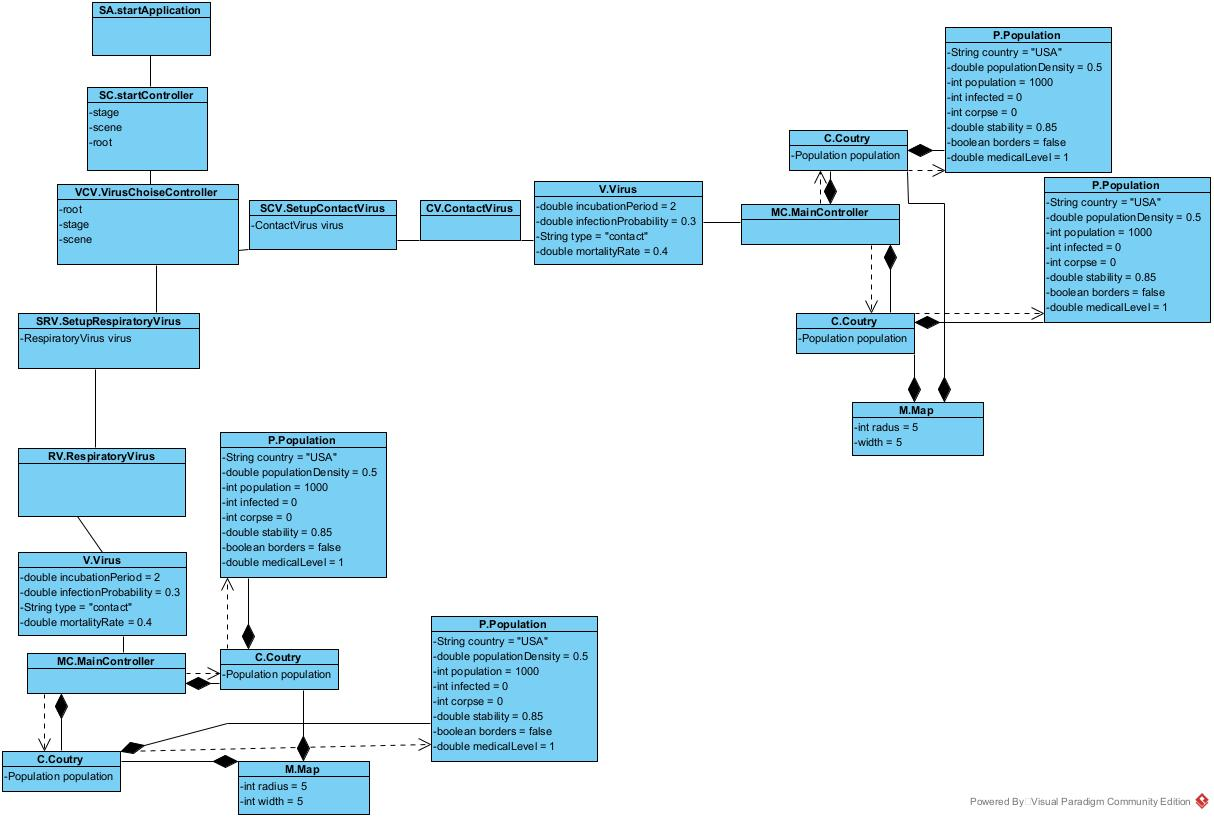
\includegraphics[width=6.6098in,height=7.05in]{a0000-img001.jpg}}


\bigskip
\bigskip
\bigskip
\bigskip
\bigskip
\bigskip
\bigskip
\bigskip
\bigskip
\bigskip
\bigskip
\bigskip
\bigskip
\bigskip
\bigskip
\begin{center}
	14
\end{center}
\bigskip


\bigskip


\bigskip

\clearpage{\centering
\textbf{Diogram klas}
\par}

\vspace{6pt}
\lfbox[margin=0mm,border-style=none,padding=0mm,vertical-align=top]{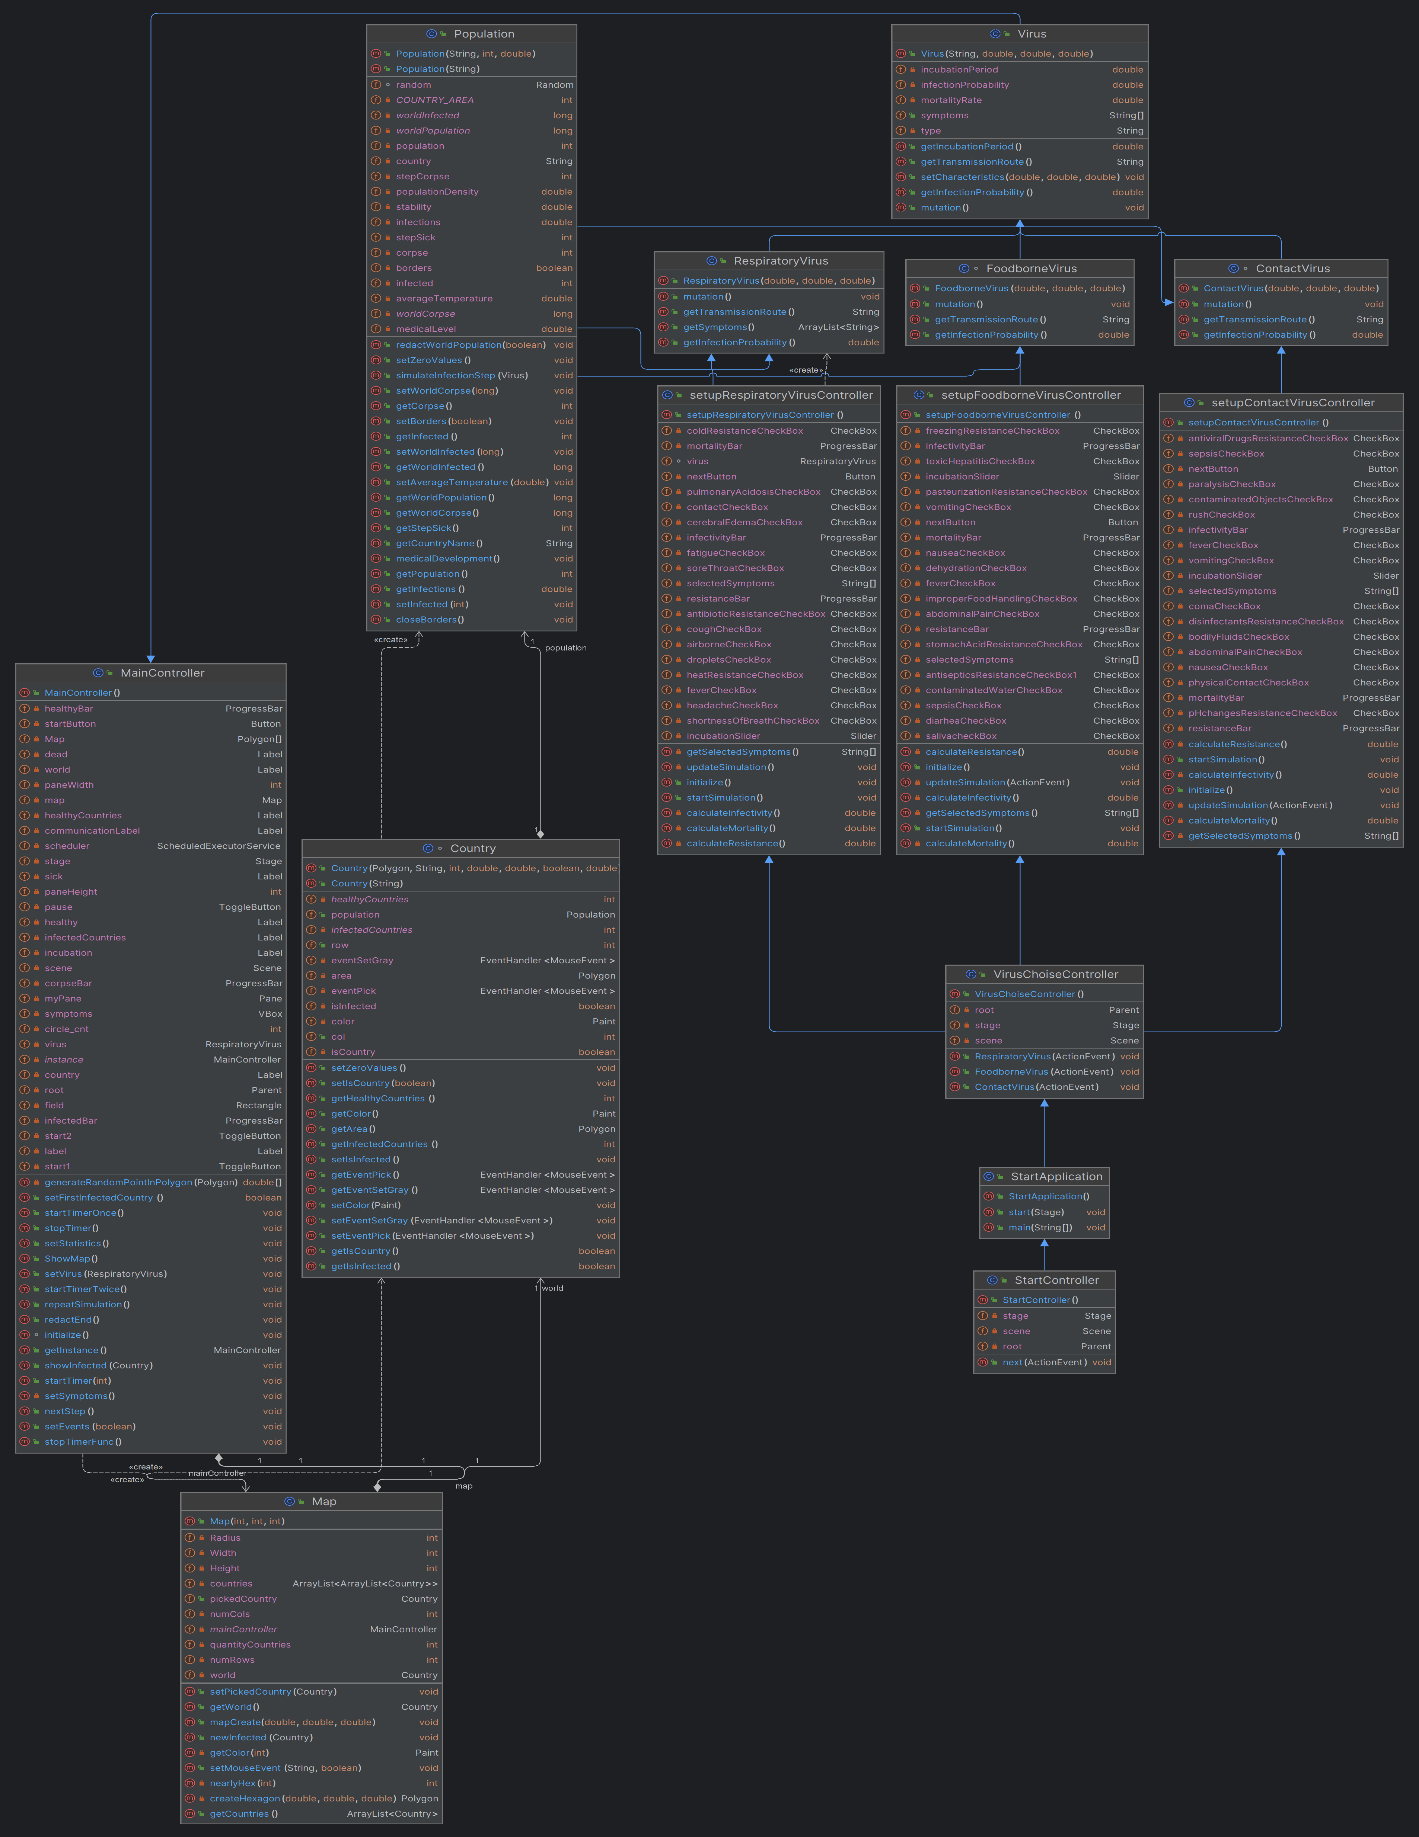
\includegraphics[width=6.448in,height=8.348in]{a0000-img002.png}}
\bigskip
\bigskip
\bigskip
\bigskip
\bigskip
\bigskip
\bigskip
\bigskip
\bigskip
\bigskip
\begin{center}
	15
\end{center}
\end{document}
